
\section{Results}


Summary stats of initial data... -highlight gaps in data


\subsection{Comparison of Hypervolumes}
Any summary stats? Maybe average/
figure - example of 'stable' hypervolume vs 'unstable' hypervolume (stable = LF, Unstable = E)



\subsection{Effect of Aboveground Biomass}

Report outcome of the ANOVAs

\begin{figure}[H]
	\centering
	\includegraphics[width=\textwidth]{figures/figure2.pdf}
	\caption{\hl{here is my caption}}
	\label{fig:2}
\end{figure}

Trees were found to on average have a significantly higher than either mammals or


\begin{figure}[H]
	\centering
	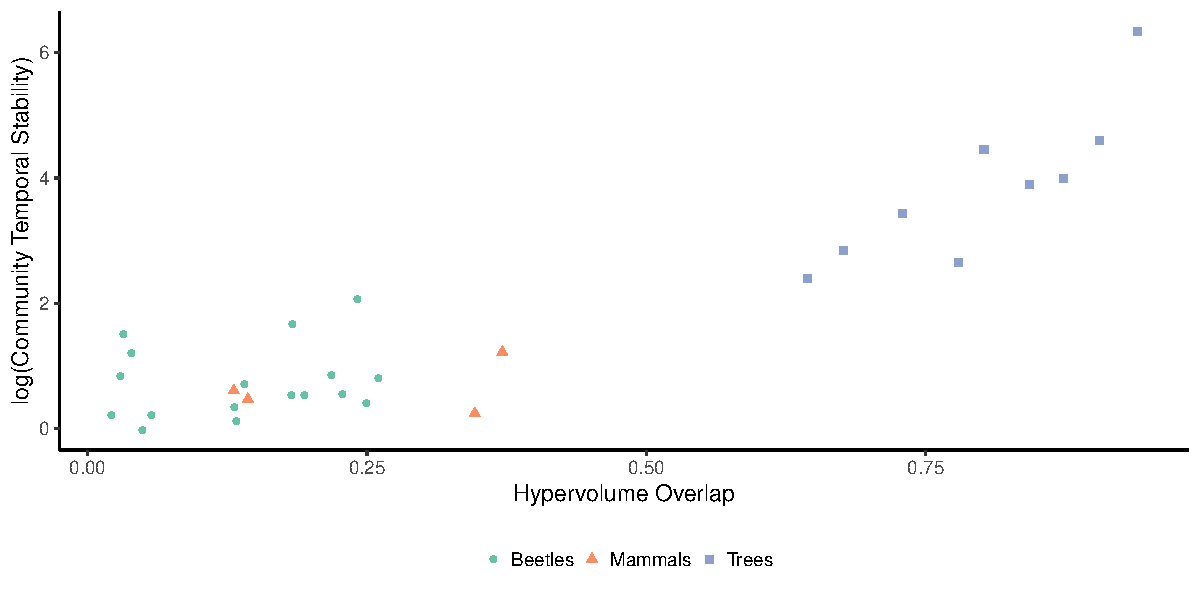
\includegraphics[width=\textwidth]{figures/figure3.pdf}
	\caption{\hl{here is my caption}}
	\label{fig:3}
\end{figure}


